%\graphicspath{{../images/}}
\section{Обзор методов шумоподавления}
\subsection{Постановка задачи}
Будем считать, что существует исходное изображение $x$, которое не искаженно шумом. После процедуры искажения шумом $n$, получаем шумное изображение $y$. Степень зашумленности изображения можно описать следующим понятием SNR.
SNR (отношение сигнал шум) - безразмерная величина, равная отношению мощности сигнала на мощность шума. В текущих обозначениях получим:
\begin{equation}
	SNR = \frac{P_y}{P_n}
\end{equation} 
где
\begin{itemize}
	\item $P_x$ - мощность сигнала (изображения)
	\item $P_n$ - мощность шума
\end{itemize}
Значит, что бы уменьшить влияния шума на изображения, необходимо либо увеличить мощность сигнала, что из-за особенностей строения устройств, детектирующих изображение, приведет к увеличению шума. Либо уменьшить количество шума. Вторым методом и занимаются алгоритмы шумоподавления.
В данной ВКР будем считать, что изображение $x$ будет искаженно аддитивным шумом $n$, искаженное изображение будет обозначаться $y$. Опишем это следующим образом.
\begin{equation}
	y = x + n
\end{equation}
Целью шумоподавления является нахождения  исходного изображения $x$, при этом слагаемое $n$ неизвестно, а доступно лишь только зашумленное изображение $y$.



\subsection{Модели шума}
Шум изображения - это случайное изменение яркости или цветовой информации на изображениях и, как правило, аспект электронного шума. Шум может как зависеть от изображения так и быть независимым. Является нежелательным побочным продуктом захвата изображения, который скрывает желаемую информацию.

Шум изображения может варьироваться от практически незаметных пятен на цифровой фотографии, сделанной при хорошем освещении, до оптических и радиоастрономических изображений, которые почти полностью представляют собой шум, из которого небольшое количество информации может быть получено с помощью сложной обработки. Такой уровень шума был бы недопустим на фотографии, так как было бы невозможно даже определить объект\cite{Noise}.

Характер проблемы удаления шума зависит от типа шума, повреждающего изображение\cite{Gonzalez}. 
\begin{itemize}
	\item Гауссовский шум
	\item Пуассоновский шум
	\item Шум Релея
	\item Шум Эрланга
	\item Импульсный шум
	\item Равномерный шум
	\item Экспоненциальный шум
\end{itemize}

Ниже будут рассмотренны одни из самых популярных моделей шума.
\subsubsection{Гауссовский  шум}
Модель гауссовского шума является одной из самых популярных моделей шума в задачах шумоподавления, так как он описывает естественные причины появления шумах, так же это обусловленно математической простотой описания данного типа шума.
Основные источники гауссовского шума в цифровых изображениях возникают во время получения, например шум датчика, вызванный плохим освещением или высокой температурой.
Гауссовский шум является аддитивным, поэтому процесс искажения цифрового изображения можно описать следующей формулой:
\begin{equation}
	y = x + n
\end{equation}
где
\begin{itemize}
	\item y - зашумленное изображение 
	\item x - исходное изображение
	\item n - случайная величина имеющая гауссовское распределение.
\end{itemize}
Гауссовский шум можно описать плотностью вероятности имеющий вид\cite{gauss}:
\begin{equation}
	P(z)=\frac{1}{\sigma\sqrt{2\pi}}e^{\frac{(z-\mu)^2}{2\sigma^2}}
\end{equation}
где
\begin{itemize}
	\item $P(z)$ - плотность вероятности
	\item $z$ - равномерно распределенная случайная величина
	\item $\sigma$ - среднеквадратичное отклонение
	\item $\mu$ - среднее значение
\end{itemize}


\subsubsection{Пуассоновский шум}
Немаловажным на практике является также пуассоновский шум, известный так же как фотонный шум. Его ожидаемая величина зависит от сигнала.
Датчики изображения измеряют освещенность сцены путем подсчета количества дискретных фотонов, падающих на датчик в течение заданного интервала времени. В цифровых датчиках фотоэффект используется для преобразования фотонов в электрон. Независимость случайных индивидуальных приходов фотонов приводит к фотонному шуму, зависящей от сигнала форме неопределенности, которая является свойством самого базового сигнала\cite{poisson}.  Количество фотонов, которые буду задетектированы описываются пуассоновским распределением.


 Распишем выражения плотности вероятности для него.
\begin{equation}
	P(X=k)=\frac{N^k}{k!}e^{-N}
\end{equation}
где:
\begin{itemize}
	\item $P(X=k)$ - плотность вероятности
	\item $X$ - случайная количество фотонов
	\item $k$ - количество фотонов, которые могут быть детектированы 
	\item $N$ - реальное количество фотонов
\end{itemize}

\subsection{Простейшие алгоритмы}
Для демонстрации работы фильтров будет использовано следующее изображение.
\begin{figure}[H]\label{img:orig}
	\center{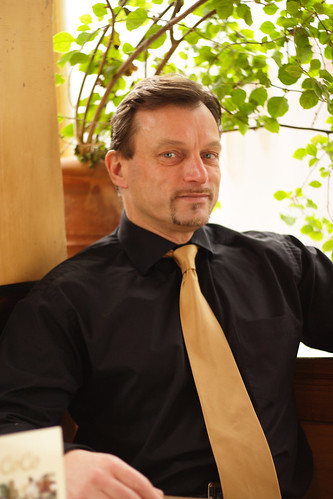
\includegraphics[scale=0.5]{orig}}
	\caption{Изображение взятое из открытой базы данных \cite{imageNet}}
\end{figure}

Всякий раз  мы будем на него накладывать аддитивный гауссовский шум с дисперсией равной  0.05.
\begin{figure}[H]\label{img:noised}
	\center{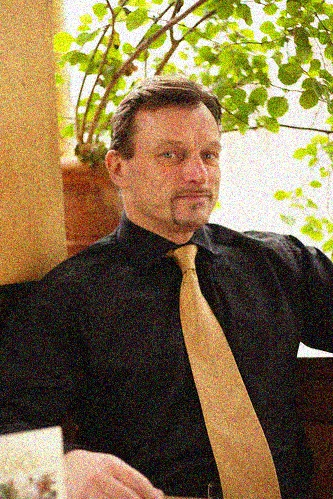
\includegraphics[scale=0.5]{noised}}
	\caption{Изображения с добавлением аддитивного гауссовского шума с $\sigma=0.05$}
\end{figure}
\subsubsection{Box фильтр}
Первые фильтры были линейными, они были основаны на идее, что пиксели в некоторой малой окрестности имеют примерно одинаковые значения интенсивности. Поэтому если представлять каждый пиксель в виде суммы пикселей в окрестности, то это поможет избавиться от шума. Такой фильтр называется "Box" фильтром. "Box" фильтра задается квадратной матрицей с радиусом r, где каждый элемент матрицы равен $\frac{1}{r^2}$.
\begin{figure}[H]
	\center{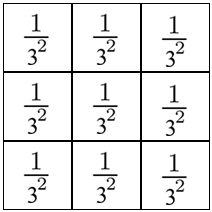
\includegraphics[scale=0.5]{kernelBox}}
	\label{img:kernelBox}
	\caption{Пример ядра "box" фильтра с радиусом 3}
\end{figure}
Ниже представлен пример работы фильтра.
\begin{figure}[H]
	\center{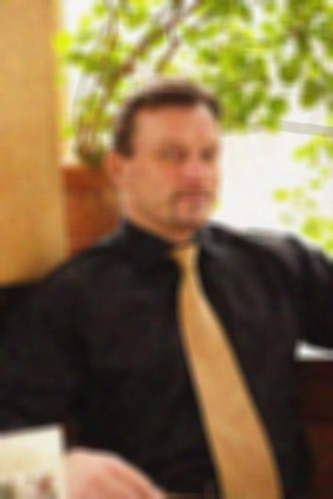
\includegraphics[scale=0.5]{box11}}
	\caption{Результат применения "box" фильтра с радиусом 11}
\end{figure}
\begin{figure}[H]
	\center{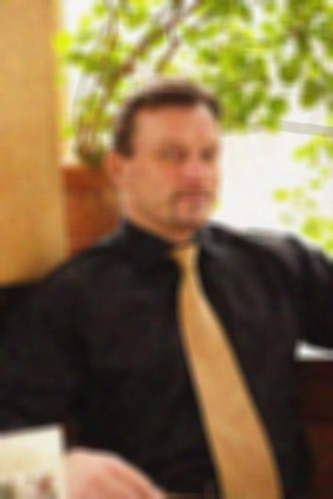
\includegraphics[trim={5cm 10cm 10cm 5cm},scale=3, clip]{box11}}
	\caption{Артефакты при применении "box" фильтра с радиусом 11}
\end{figure}
Как можно видеть, результат работы "box"  фильтра имеет артефакты в виде горизонтальных и вертикальных линий. Это является причиной почему данный фильтр не используют на практике.
\subsubsection{Гауссовский фильтр}
Улучшением идеи "Box"  фильтра стал гауссов фильтр. В отличии от ядра "box" фильтра, значения ядра гауссовского фильтра вычисляются с помощью функции гаусса от двух переменных :

\begin{equation}
	G(x,y) = \frac{1}{\sqrt{2\pi}\sigma^2}e^{\frac{x^2+y^2}{2\sigma^2}}
\end{equation}
где
\begin{itemize}
	\item $x,y$ - координаты ядра
	\item $\sigma$ среднеквадратичное отклонение
\end{itemize}

Параметр $\sigma$ обозначает насколько сильно будет размыто изображение, соотвественно от $\sigma$ зависит и радиус ядра фильтра. Т.е. $r=3\sigma$. Ниже представлены графики одномерное функции гаусса с различными значениями $\sigma$.

\begin{figure}[H]
	\center{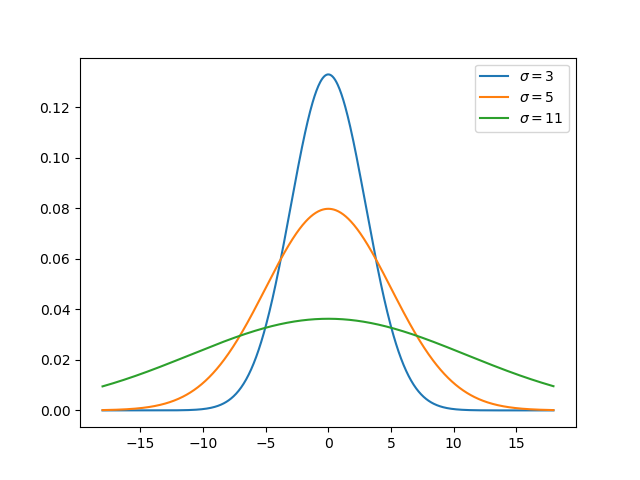
\includegraphics[draft]{plotGauss.png}}
	\caption{Графики функции гаусса с параметром $\sigma = 3,5,11$}
\end{figure}

Применим фильтр гаусса для рис. \ref{img:orig} с различными параметрами $\sigma$.

\begin{figure}[h]
	\centering \subfigure[]{
\includegraphics[scale=0.5]{gauss3.png}
		\label{img:gauss3}
	}
	\hspace{4ex}
	\subfigure[]{
\includegraphics[scale=0.5]{gauss11.png}
		\label{img:gauss11}
	}
	\caption{Пример работы гауссовского фильтра: \subref{img:gauss3} с радиусом 3; \subref{img:gauss11} с радиусом 11}
\end{figure}

\paragraph{Достоинства и недостатки "box" фильтра и фильтра гаусса}

Преимуществом первых фильтров является простая реализация и быстрая скорость работы. Так как процесс шумоподавления, можно представить в виде поэлементного умножения спектрального образа шума на спектральный образ изображения. Но они также обладают одним существенным недостатком. Данные фильтры размывают края, это может негативно сказываться на алгоритмах компьютерного зрения.
\subsubsection{Медианный фильтр}
Избавиться от указанного выше недостатка попытался медианный фильтр. Он основан на той идее, что пиксели в некоторой малой окрестности имеют приблизительно равную интенсивность, а шум, соотвественно сильно отличается. Поэтому для пикселя, для которого вычисляется новое значения, берутся пиксели в некоторой окрестности. Как правило, это квадрат с радиусом r. Данные пиксели сортируются по возрастанию или убыванию и новым значением объявляется то, что находится в середине.

Продемонстрируем на примере работу фильтра.

\begin{figure}[H]
\centering \subfigure[]{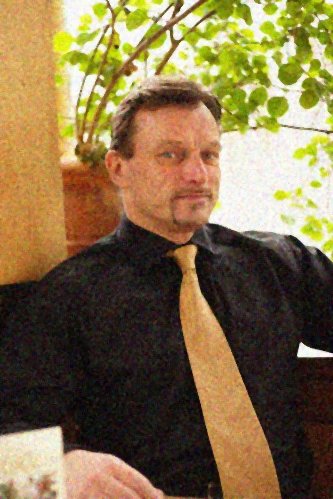
\includegraphics[scale=0.5]{median3.png}
		\label{img:median3}
	}
\hspace{4ex}
\subfigure[]{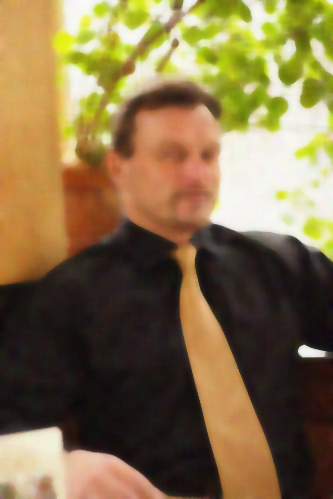
\includegraphics[scale=0.5]{median11.png}
	\label{img:median11}
}
	\caption{Результат работы медианного фильтра: \subref{img:median3} с радиусом 3; \subref{img:median11} с радиусом 11}
\end{figure}
\paragraph{Достоинства и недостатки медианного фильтра}
Данный алгоритм работает хорошо, только с импульсным шумом, что сильно ограничивает его область использования. Но главным недостатком фильтра является то, что изображение теряет своё визуальное качество.
